\documentclass{cmc}
\usepackage{makecell}
\begin{document}

\pagestyle{fancy}
\lhead{\textit{\textbf{Computational Motor Control, Spring 2022} \\
    Final project, Project 1, GRADED}} \rhead{Student \\ Names}

\section*{Student names: \ldots (please update)}

\textit{Instructions: Update this file (or recreate a similar one, e.g.\ in
  Word) to prepare your answers to the questions. Feel free to add text,
  equations and figures as needed. Hand-written notes, e.g.\ for the development
  of equations, can also be included e.g.\ as pictures (from your cell phone or
  from a scanner).  \textbf{\corr{This lab is graded.}} and needs to be
  submitted before the \textbf{\corr{Deadline : Wednesday 18-05-2022 23:59. You
      only need to submit one final report for all of the following exercises
      combined henceforth.}} Please submit both the source file (*.doc/*.tex)
  and a pdf of your document, as well as all the used and updated Python
  functions in a single zipped file called
  \corr{final\_report\_name1\_name2\_name3.zip} where name\# are the team
  member’s last names.  \corr{Please submit only one report per team!}}
\\

\section*{Swimming with Salamandra robotica – CPG Model}
\label{sec:exploring-swimming}

In this project you will control a salamander-like robot Salamandra
robotica II for which you will use Python and the MuJoCo physics
engine. You have an opportunity to use what you’ve learned until
now to make the robot swim and walk in open and closed loop scenarios.
In order to do this, you should implement a CPG based swimming controller,
similarly to the architecture shown in Figure~\ref{fig:controller-model}.

The project is based on the research of~\cite{Crespi2013},
~\cite{Karakasiliotis2013},~\cite{ijspeert2007swimming}
and~\cite{thandiackal2021emergence}. It is strongly recommended to
review~\cite{ijspeert2007swimming},~\cite{thandiackal2021emergence} and their
supplementary material provided on the Moodle.
You will be tasked with replicating and studying the
Central Pattern Generator (CPG) network proposed in those papers.

\begin{figure}[h]
  \centering
  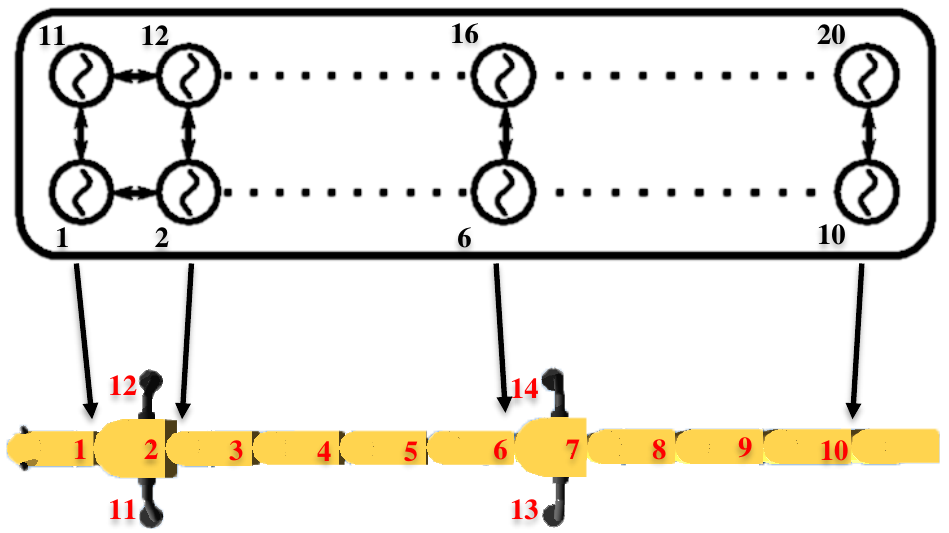
\includegraphics[width=0.5\textwidth]{figures/model_controller.png}
  \caption[Controller model]{A double chain of oscillators controlling
    the robot’s spine.}
  \label{fig:controller-model}
\end{figure}

\begin{figure}[ht]
  \centering 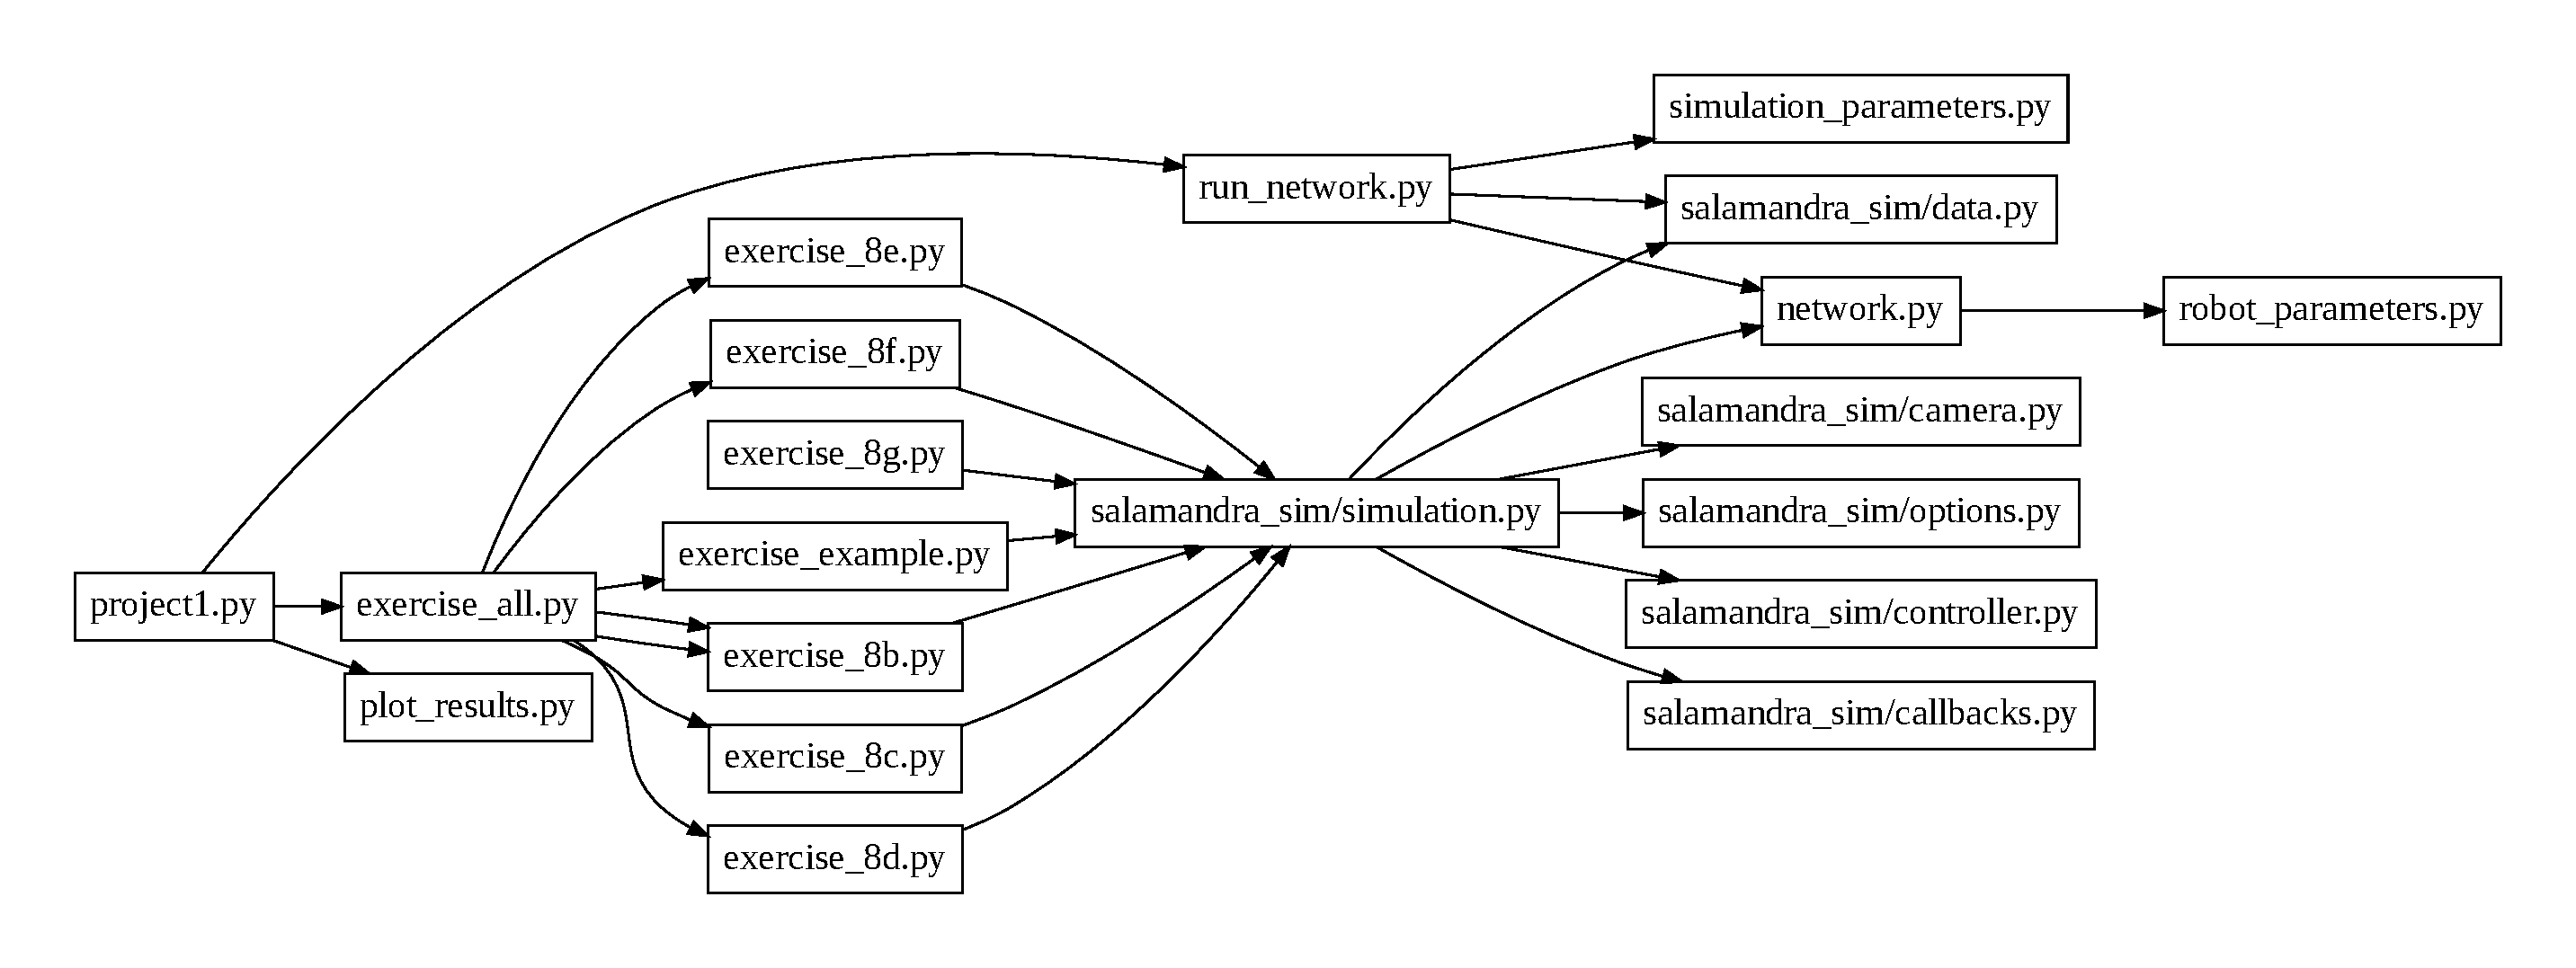
\includegraphics[width=1.0\textwidth]{figures/files}
  \caption{\label{fig:files} Exercise files dependencies. In this lab, you will
    be modifying \fileref{run\_network.py}, \fileref{network.py},
    \fileref{robot\_parameters.py} and \fileref{simulation\_parameters.py}}
\end{figure}

% \newpage

\subsection*{Code organization}
\label{subsec:code}

\begin{itemize}
\item \corr{\textbf{project1.py}} - A convenient file for running the entire
  project. Note you can also run the different exercises in parallel by
  activating \texttt{parallel=True}. \textit{You do not need to modify this
    file.}
\item \corr{\textbf{exercise\_all.py}} - Another convenient file for running all
  or specified exercises depending on arguments provided. \textit{You do not
    need to modify this file.}
\item \corr{\textbf{network.py}} - This file contains the different classes and
  functions for the CPG network and the Ordinary Differential Equations
  (ODEs). You can implement the network parameters and the ODEs here. Note that
  some parameters can be obtained from robot\_parameters.py to help you control
  the values.
\item \corr{\textbf{robot\_parameters.py}} - This file contains the different
  classes and functions for the parameters of the robot, including the CPG
  network parameters. You can implement the network parameters here. Note that
  some parameters can be obtained from the SimulationParameters class in
  \corr{simulation\_parameters.py} and provided in \corr{exercise\_\#.py} to
  help you control the values (refer to example.py).
\item \corr{\textbf{simulation\_parameters.py}} - This file contains the
  SimulationParameters class and is provided for convenience to send parameters
  to the setup of the network in \corr{network.py::SalamandraNetwork} via the
  robot parameters in \corr{robot\_parameters.py::RobotParameters}. The
  SimulationParameters is also intended to be used for experiment-specific
  parameters for the exercises. All the values provided in SimulationParameters
  are logged for each simulation, so you can also reload these parameters when
  analyzing the results of an experiment.
\item \corr{\textbf{run\_network.py}} - By running the script from Python,
  MuJoCo will be bypassed and you will run the network without a physics
  simulation. Make sure to use this file for question 8a to help you with
  setting up the CPG network equations and parameters and to analyze its
  behavior. This is useful for debugging purposes and rapid controller
  development since running the MuJoCo simulation takes more time.
\item \corr{\textbf{exercise\_example.py}} - Contains the example code structure
  to help you familiarize with the other exercises. \textit{You do not need to
    modify this file.}
\item \corr{\textbf{exercise\_\#.py}} - To be used to implement and answer the
  respective exercise questions. Note that \corr{exercise\_example.py} is
  provided as an example to show how to run a parameter sweep. Note that network
  parameters can be provided here.
\item \corr{\textbf{exercise\_all.py}} - A convenient file for running different
  exercises depending on arguments. See \corr{\textbf{project1.py}} for an example
  on how to call it. \textit{You do not need to modify this file.}
\item \corr{\textbf{plot\_results.py}} - Use this file to load and plot the
  results from the simulation. This code runs with the original example provided
  and provides examples on how to collect the data.
\item \corr{\textbf{salamandra\_simulation folder}} - Contains all the remaining
  scripts for setting up and running the simulation experiments. \textit{You do
    not need to modify any of these file but should still go through them to get
    a better understanding of the code.}
\end{itemize}

% \newpage

\section*{Prerequisites}
To have all the necessary python packages necessary to complete the
final project, do the following.

Pull the latest version of the exercise repository. Navigate to the
location of your repository in the terminal and execute the following,

\begin{lstlisting}[language=Bash]
  >> pip install -r requirements.txt
\end{lstlisting}

To install the simulator, please follow the instructions in Lab6.

\subsection*{Running the simulation}
You can run a simulation example with \corr{\textbf{exercise\_example.py}}. You
should see the Salamandra robotica model floating on the water. At this point
you can now start to work on implementing your exercises. Note that it is still
possible to proceed with exercise 8a if the simulator is not installed yet.

\newpage

\section*{Questions}

The exercises are organized such that you will have to first implement the
oscillator network model in \corr{run\_network.py} code and analyze it before
connecting it to the body in the physics simulation.  Exercise 8a describes the
questions needed to implement the oscillator models. After completing exercise
8a you should have an oscillator network including both the spinal CPG and limb
CPG. Using the network implemented in exercise 8a you can explore its
capability to perform swimming. You will then extend the network to account
for the presence of exterosensory feedback due to the hydrodynamic forces
acting on the body of the network. You will show that a chain of uncoupled
oscillators with sensory feedback is still able to reproduce a travelling wave.
You will also study the interplay between open loop and closed loop
behavior to optimize the swimming gait according to speed and energetic cost.
Finally, you will study the robustness of the different configurations with
respect to disruptions of couplings, oscillators and sensors.
Exercises 8b to 8g will be performed with a Salamandra robotica II model using
the MuJoCo simulation.

%%%%%%%%%%%%%%%%%%%%%%%%%%%%%%%%%%%%%%%%%%%%%%%%%%%%%%%%%%%%%%%%%%%%%%%%%%%%%%%%%%%%%%%%%%%%%%%%%%%%

\subsection*{8a. Implement a double chain of oscillators along with
  limb CPG's}
\label{sec:implement-chain}

Salamandra robotica has 8 joints along its spine and 1 joint for each
limb. The controller is defined as

\begin{equation}
  \label{eq:dphase}
  \dot{\theta}_i = 2 \pi f + \sum_j r_j w_{ij} sin(\theta_j - \theta_i - \phi_{ij})
\end{equation}

\begin{equation}
  \label{eq:dr}
  \dot{r}_i = a (R_i - r_i)
\end{equation}

\begin{equation}
  \label{eq:output}
  q_i = r_i(1 + cos(\theta_i)) - r_{i+8}(1 + cos(\theta_{i+8})) \text{ if body joint}
\end{equation}

with $ \theta_i $ the oscillator phase, f the frequency, $ w_{ij} $ the coupling
weights, $ \phi_{ij} $ the nominal phase lag (phase bias), $ r_i $ the
oscillator amplitude, $ R_i $ the nominal amplitude, $ a $ the convergence
factor and $ q_i $ the spinal joint angles. For more information, please refer
to \cite{ijspeert2007swimming}. Also note how these are the same equations,
although Equation \eqref{eq:dr} has been simplified into a first order ODE in
order to simplify the implementation in this project.

\begin{enumerate}
\item Implement the double chain oscillator model using the functions
  \fileref{network.py::network\_ode}. Test your implementation by running the
  network using \fileref{run\_network.py}. For the network parameters check
  lecture slides (pay attention to different number of segments). You can also
  find more information in~\cite{ijspeert2007swimming} (especially in the
  supplementary material). You can set all the network parameters in the
  \fileref{robot\_parameters.py::RobotParameters}. To facilitate your work, you
  could start by only implementing the network for the body oscillators
  ($i=[0, ..., 15]$) and ignoring the leg oscillators ($i=[16, ..., 20]$). Refer
  to \corr{salamandra\_simulation/data.py::SalamandraState} and
  \corr{robot\_parameters.py::}\-\corr{RobotParameters} for the dimensions of
  the state and the network parameters respectively.

\item Implement the output of your CPG network to generate the spinal joint
  angles according to equation~\ref{eq:output}. Implement this in the function
  \fileref{network.py::motor\_output}. Verify your implementation in by running
  the Python file \fileref{run\_network.py}.


\item Implement a drive and show that your network can generate swimming and
  walking patterns similarly to~\cite{ijspeert2007swimming}. Try to reproduce
  the plots in~\ref{fig:science_oscillator_patterns} and
~\ref{fig:science_oscillator_properties}


  \textbf{Hint:} The state for the network ODE is of size 40 where the first 20
  elements correspond to the oscillator phases $\theta_i$ of the oscillators and
  the last 24 elements correspond to the amplitude $r_i$. The initial state is
  set in the init of \corr{network.py::SalamanderNetwork}.
\end{enumerate}

\begin{figure}[H]
  \centering
  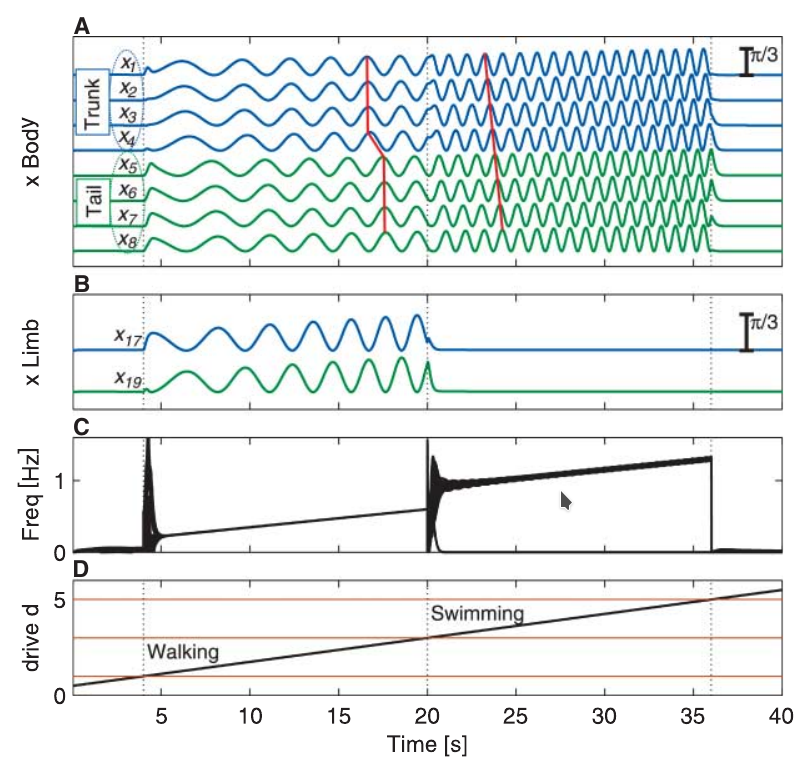
\includegraphics[width=0.7\textwidth]{figures/science_oscillator_patterns}
  \caption{Oscillator patterns from \cite{ijspeert2007swimming}, see
    \cite{ijspeert2007swimming} for details}
  \label{fig:science_oscillator_patterns}
\end{figure}

\begin{figure}[H]
  \centering
  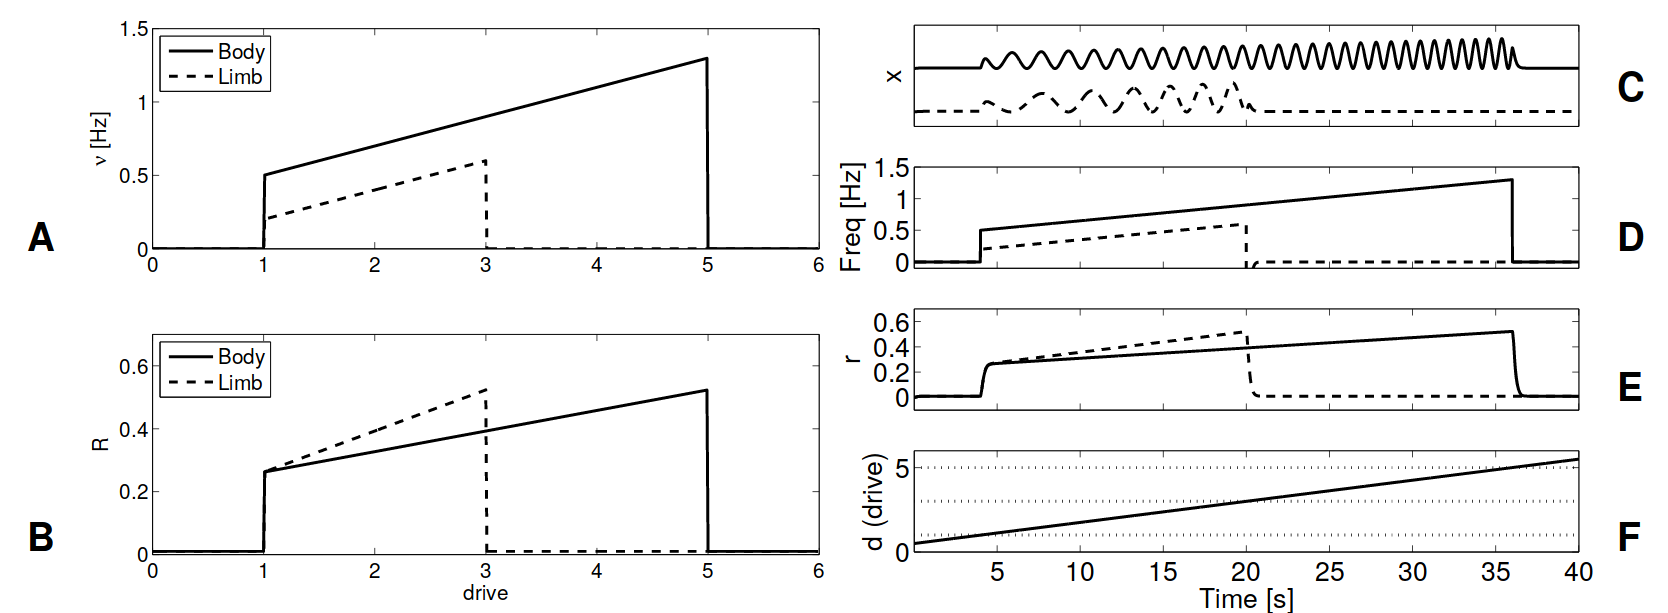
\includegraphics[width=1.0\textwidth]{figures/science_oscillator_properties}
  \caption{Oscillator properties from \cite{ijspeert2007swimming} supplementary
    material, see \cite{ijspeert2007swimming} for details}
  \label{fig:science_oscillator_properties}
\end{figure}


%%%%%%%%%%%%%%%%%%%%%%%%%%%%%%%%%%%%%%%%%%%%%%%%%%%%%%%%%%%%%%%%%%%%%%%%%%%%%%%%%%%%%%%%%%%%%%%%%%%%

\subsection*{8b. Effects of amplitude and phase lags on swimming
  performance}
\label{sec:amplitude-phase-performance}

Now that you have implemented the controller, it is time to run experiments to
study its behaviour. How does phase lag and oscillation amplitude influence the
speed and energy? Use the provided \corr{exercise\_8b.py} to run a grid search
to explore the robot behavior for different combinations of amplitudes and phase
lags. Use \corr{plot\_results.py} to load and plot the logged data from the
simulation. Include 2D/3D plots showing your grid search results and discuss
them. How do your findings compare to the wavelengths observed in the
salamander?

% Run the grid search twice, for frequencies of 1Hz and 2Hz.

\begin{itemize}
\item \textbf{Hint 1:} To use the grid search, check out the example provided in
  \corr{exercise\_example.py}. This function takes the desired parameters as a
  list of SimulationParameters objects (found in
  \corr{simulation\_parameters.py}) and runs the simulation. Note that the
  results are logged as simulation\_\#.h5 in a specified log folder. After the
  grid search finishes, the simulation will close.
\item \textbf{Hint 2:} An example of how to load and visualise grid search
  results is already implemented in \corr{plot\_results.py::main()}. Pay
  attention to the name of the folder and the log files you are loading. Before
  starting a new grid search, change the name of the logs destination folder
  where the results will be stored. In case a grid search failed, it may be
  safer to delete the previous logs to avoid influencing new results by mistake.
\item \textbf{Hint 3:} Estimate how long it will take to finish the grid
  search. Our suggestion is to choose wisely lower and upper limits of parameter
  vectors and choose a reasonable number of samples. To speed-up a simulation,
  make sure to run the simulation in fast mode and without GUI as shown in
  \corr{exercise\_example.py} or using \texttt{--fast} and \texttt{--headless}
  in the Python command line (Use \texttt{--help} for more information).
\item \textbf{Hint 4:} Energy can be estimated by integrating the product of
  instantaneous joint velocities and torques. Feel free to propose your own
  energy metrics, just make sure to include a justification for the one chosen.
\end{itemize}


%%%%%%%%%%%%%%%%%%%%%%%%%%%%%%%%%%%%%%%%%%%%%%%%%%%%%%%%%%%%%%%%%%%%%%%%%%%%%%%%%%%%%%%%%%%%%%%%%%%%

\subsection*{8c. Amplitude gradient}
\label{sec:amplitude-gradient}

\begin{enumerate}
\item So far we considered constant undulation amplitudes along the body for
  swimming. Implement a linear distribution of amplitudes along the spine,
  parametrized with two parameters: amplitudes of the first (Rhead) and last
  (Rtail) oscillator in the spine (corresponding to the first and last
  motor). To do so, you can add a parameter amplitudes=[Rhead, Rtail] in
  \corr{simulation\_parameters.py::SimulationParameters}. Don't forget to modify
  \corr{robot\_parameters.py::}\-\corr{RobotParameters::set\_nominal\_amplitudes()}
  and interpolate the amplitude gradient between values Rhead and Rtail within
  the function. Note that you can then provide this amplitudes parameter from
  \corr{exercise\_8c.py}.
\item Run a grid search over different values of parameters Rhead and Rtail (use
  the same range for both parameters). How does the amplitude gradient influence
  swimming performance (speed, energy)?  Include 3D plots showing your grid
  search results. Do it once, for frequency 1Hz and total phase lag of $2\pi$
  along the spine.
\item How is the salamander moving (with respect to different body amplitudes)?
  How do your findings in 2) compare to body deformations in the salamander?
  Based on your explorations, what could be possible explanations why the
  salamander moves the way it does?
\end{enumerate}


%%%%%%%%%%%%%%%%%%%%%%%%%%%%%%%%%%%%%%%%%%%%%%%%%%%%%%%%%%%%%%%%%%%%%%%%%%%%%%%%%%%%%%%%%%%%%%%%%%%%
\subsection*{8d. Turning and backwards swimming}
\label{sec:turning-backwards}

\begin{enumerate}
\item How do you need to modulate the CPG network (\corr{network.py}) in order
  to induce turning?  Implement this in the model and plot example GPS
  trajectories and spine angles.
\item How could you let the robot swim backwards? Explain and plot example GPS
  trajectories and spine angles.
\end{enumerate}


%%%%%%%%%%%%%%%%%%%%%%%%%%%%%%%%%%%%%%%%%%%%%%%%%%%%%%%%%%%%%%%%%%%%%%%%%%%%%%%%%%%%%%%%%%%%%%%%%%%%

\subsection*{8e. Exterosensory feedback}
\label{sec:exterosensory-feedback}

So far we considered constant undulation amplitudes obtained as a result
of an open loop control from the central pattern generators.
Taking inspiration from~\cite{thandiackal2021emergence}, you can extend the
current model to account for the effect of feedback due to the
hydrodynamic forces acting on the body during swimming.
The model can be extended as follows:

\begin{equation}
  \label{eq:dphase_fb}
  \dot{\theta}_i = 2 \pi f + \sum_j r_j w_{ij} \sin(\theta_j - \theta_i - \phi_{ij})
                  + \corr{w_{fb} F_{i} \cos(\theta_i)}
\end{equation}

\begin{equation}
  \label{eq:dr_fb}
  \dot{r}_i = a (R_i - r_i)
\end{equation}

\begin{equation}
  \label{eq:output_fb}
  q_i = r_i(1 + \cos(\theta_i)) - r_{i+8}(1 + \cos(\theta_{i+8})) \text{ if body joint}
\end{equation}

where $ F_{i} $ is the normal hydrodynamic force acting on the i-th link and
$ w_{fb} $ is a gain linking the mechanical and neuronal input.

\begin{enumerate}
\item Implement a double chain oscillator model whithout couplings between
  adjactent segments. Is the network still capable of producing a swimming
  behavior?

\item Starting from the previous step, include the contribution of sensory
  feedback. What is its effect on the decoupled network? Is it possible to find
  a parameters' configuration that allows for the creation of a characteristic
  travelling wave? How does the current model perform compared to the
  open loop one?  Which are the differences in terms of speed and power
  consumptions?

\textbf{Hint 1:} The couplings between segments and hemisegments can be
  accessed from \corr{SimulationParameters}.

\textbf{Hint 1:} The initial phase of the oscillators can be
  set with the \corr{initial\_phases} argument to \corr{simulation}.

\textbf{Hint 2:} The loads on the body can be
  accessed in \corr{controller.py::SalamandraController::step},
  through \corr{self.animat\_data.sensors.hydrodynamics.array}.
  The aforementioned array contains all the hydrodynamic loads acting on
  each link of the model at every timestep. The six loads are ordered as
  $[ F_x, F_y, F_z, \tau_x, \tau_y, \tau_z ]$, where the x
  axis is aligned with the body link and the z axis is pointing upwards.

\end{enumerate}


%%%%%%%%%%%%%%%%%%%%%%%%%%%%%%%%%%%%%%%%%%%%%%%%%%%%%%%%%%%%%%%%%%%%%%%%%%%%%%%%%%%%%%%%%%%%%%%%%%%%

\subsection*{8f. Exploiting redundancy}
\label{sec:exploiting-redundancy}

We have previously shown the potential of sensory feedback for
substituting local connections between adjacent segments. We will now
consider a model including both sensory feedback and ascending/descending
connections.

\begin{enumerate}

\item Perform a grid search with respect to the intersegmental couplings and
the strength of the sensory feedback gain, in order to study the performance
of the overall network.

\item Describe the results you observed so far. Which network type displayed
the best performance? How do you explain the observed results?

\textbf{Hint 1:} Select values of amplitude, phase bias and drive that are
  consistent with the consideration you made in the previous exercises.

\end{enumerate}


%%%%%%%%%%%%%%%%%%%%%%%%%%%%%%%%%%%%%%%%%%%%%%%%%%%%%%%%%%%%%%%%%%%%%%%%%%%%%%%%%%%%%%%%%%%%%%%%%%%%

\subsection*{8g. Robustness to disruptions}
\label{sec:disruptions-robustness}

The models analyzed so far have been shown capable, with different performance,
to display a swimming behavior. We will now analyze their robustness to
different neural disruption.

\begin{enumerate}

  \item Consider the three networks proposed so far (CPG only,
  Decoupled segments, Combined) and implement different neural disruptions
  as proposed in~\cite{thandiackal2021emergence}. What is their effect on
  the swimming performance?

  \item Which network showed the highest robustness to disruptions?
  Explain the results you observed and their implications
  on salamander locomotion.

  \textbf{Hint:} The properties of the controller are defined and updated in
    \corr{robot\_parameters.py}. You are free to create internal variables
    that allow to selectively silence the effects of oscillators, couplings
    and sensory feedback.

  \textbf{Hint:} To ensure a fair comparison between the models, start with
  configurations showing similar performance.

  \end{enumerate}


%%%%%%%%%%%%%%%%%%%%%%%%%%%%%%%%%%%%%%%%%%%%%%%%%%%%%%%%%%%%%%%%%%%%%%%%%%%%%%%%%%%%%%%%%%%%%%%%%%%%

% \newpage

\bibliographystyle{ieeetr}
\bibliography{project1}
\label{sec:references}

% \newpage

% \section*{APPENDIX}
% \label{sec:appendix}

\end{document}

%%% Local Variables:
%%% mode: latex
%%% TeX-master: t
%%% End: